\documentclass{article}
\usepackage{graphicx}

\title{Devoir de Programmation : Tries}
\author{Marco PONTI\\ Nicolas SERRES}
\date{December 2016}

\begin{document}

\maketitle

\newpage

\section{Introduction}

Dans ce Devoir de Programmation, l'objectif est d'impl\'ementer et de comparer les
deux structures d'arbres de Patricia-Tries et de Hybride-Tries, afin de
d\'eterminer lequel est meilleur.\\

\section{Choix de la Structure}

\paragraph{Le Patricia-Tries\\\\}

Lors de l'impl\'ementation de cet algorithme un probl\`eme c'est pos\'e, le
choix de la structure.\\

Premi\`erement, la structure \'etait un objet compos\'e d'un pr\'efixe et d'un vecteur de
caract\`ere ainsi que d'un second vecteur contenant des pointeurs vers les
Patricia-tries fils, le probl\`eme \'etant la taille du vecteur en m\'emoire ainsi que
le nombre de pointeur vers null. De plus, en java, un caract\`ere ne peut etre mis
\`a null, une simple modification aurait \'et\'e de changer le vecteur de caract\`ere en
vecteur de chaine, mais la m\'emoire restait un probl\`eme.\\

La seconde \'etait d'utiliser des Array-list, mais cela allait \`a l'encontre des
arbres et des exemples montr\'es par les nos professeurs, de plus la complexit\'e en
pire cas aurait \'et\'e de parcourir chaque caract\`eres * la profondeur.\\

La troisi\`eme structure impl\'ement\'ee a \'et\'e une simple hash-map avec comme cl\'e le
pr\'efixe et en valeur un Patricia-Tries, malheureusement cette structure a \'et\'e
abandonn\'e, car elle forçait la plupart des algorithmes \`a devoir parcourir toute
les cl\'es de la hash-map comme le dernier algorithme ce qui faisait perdre tout
l'int\'eret d'utiliser des hash-map.\\

La derni\`ere impl\'ementation, donc celle utilis\'ee dans notre code, est un pr\'efixe
avec une hash-map compos\'e de cl\'es valant la premi\`ere lettre du pr\'efixe du fils
et en valeur le fils.\\
L'arbre initial poss\`ede pour racine le mot vide, la structure ne pr\'esente aucun pointeur
vers null, car tous les Patricias-Tries sont cr\'e\'es s'il y a l'existence d'une
lettres et la hash-map est cr\'e\'e par d\'efauts meme s'il se trouve etre vide.\\

Explication de la fonction de fusion :\\
La fonction parcours les deux arbres chacun au m\^eme niveau et test si
les pr\'efixes sont similaires.\\
Si oui elle ins\`ere chaque cl\'e n'\'etant pas pr\'esente dans le premier arbre dans
celui-ci, si elle existe, la fonction de fusion est alors lanc\'ee sur les deux
fils.\\
Si les pr\'efixes sont diff\'erents, la fonction s\'epare les pr\'efixes en deux parties
la racine commune et le reste des deux pr\'efixes, puis une r\'ecursion est lanc\'ee
sur le nouveau noeud de la racine commune.\\

Exemple graphique d'un Patricia-Tries avec les mots :\\
arbre, arbuste, arc, artiste, destin et magique\\

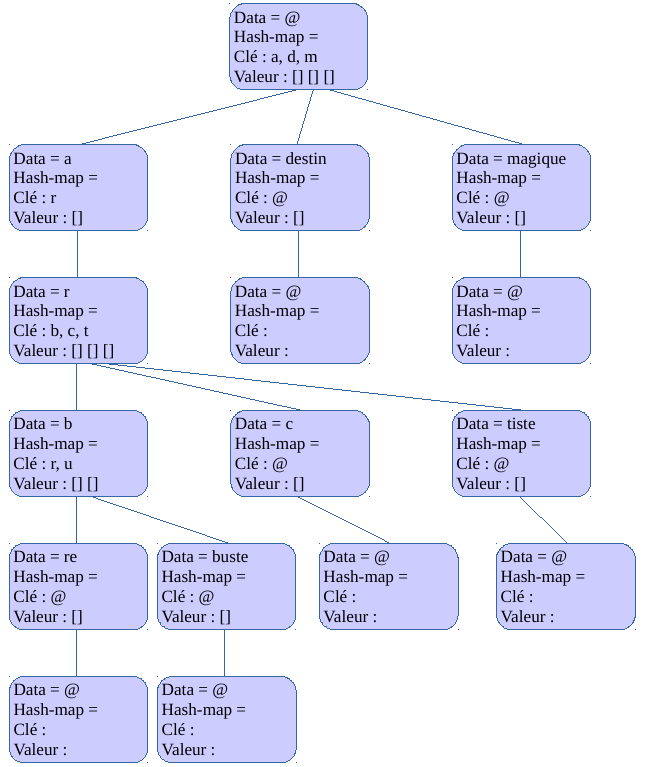
\includegraphics[scale=0.5]{graphicc.png}

\newpage

\paragraph{Le Hybride-Tries\\\\}


Chaque noeud hybride est constitu\'e d'une lettre, d'un bollean pour savoir si on 
est a la fin d'un mot, d'un fil et de 2 freres.\\
Lorsque qu'un noeud a une lettre \'egale a null c'est que l'arbre est vide.\\

L'impl\'ementation est ensuite en accord avec la structure des tries hybrides vu 
en cours.\\

Toutes les fonctions qui n\'ecessitent de parcourir l'arbre utilise la r\'ecursivit\'e 
afin d'avoir le code le plus simple possible.\\

Pour les fonctions avec un d\'eplacement sp\'ecial, il est expliqu\'e directement dans
 le code par des commentaires.\\

La fonction de r\'e\'equilibrage est a d\'etaill\'ee :\\
Le r\'e\'equilibrage d'un trie hybride peut se faire au niveau des freres en les
consid\'erants comme des noeuds qu'on pourrait disposer de facon a obtenir un
arbre complet.\\
Pour voir si les freres sont d\'es\'equilibr\'es (cf. ne forme pas un arbre complet)
on regarde si la profondeur totale des freres est sup\'erieure au log en base 2 du
nombre de frere.\\
- ligne 604 : if (profondeurMaxFrere>Math.abs(log2(nbFrere)))\\
Dans ce cas la, on appel listesFrereSorted qui r\'ecupere tous les freres, supprime
leur lien frereGauche et frereDroit, puis les classe par ordre de leur lettre.\\
Puis on renvoie reformeFrere qui s'occupe de replacer les noeuds dans un arbre
complet.\\
reformeFrere prenant à chaque fois le milieu de la liste avec pour frere gauche
le milieu de la liste gauche et pour frere droit le milieu de la liste droite.\\
On effectue ce test de r\'e\'equilibrage pour chaque liste de frere c'est a dire a
chauque d\'eplacement vers le bas dans l'arbre :\\
- arbre.fils= reequilibrageFrere(arbre.fils);\\

\newpage

Hybrid-Tries avant r\'e\'equilibrage\\\\
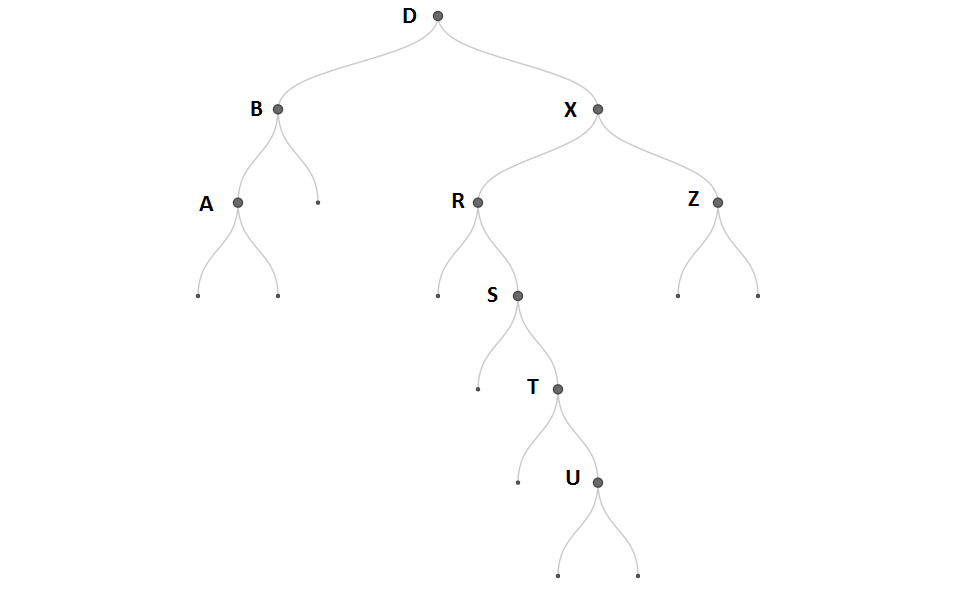
\includegraphics[scale=0.5]{HybBefore.png}
\\\\
Hybrid-Tries apr\`es r\'e\'equilibrage\\\\
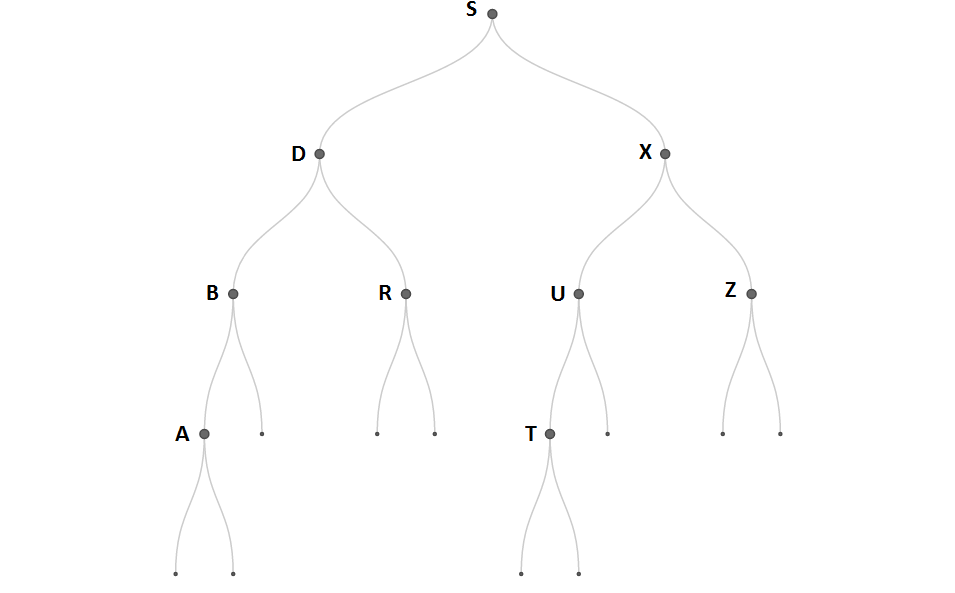
\includegraphics[scale=0.5]{HybAfter.png}

\newpage

\section{R\'eponse aux Questions}

\paragraph{Question 1.1 : }

Le caract\`ere pour le fin d'un mot est '@'

\paragraph{Question 3.9 :}

On peut reequilibrer un trie hybride au niveau des freres.
En effet si l'arbre est parfaitement \'equilibre tous les frere d'un meme noeud
formerons un arbre binaire complet. C'est en ce basant sur cette logique qu'on
trouve que le seuil est d\'epass\'e lorsque la profondeur max des freres
est sup\'erieure a la valeure absolue du log en base 2 du nombre total de frere.\\

\paragraph{Question 4.10 :}

Calcule des complexit\'ees PatriciaTrie :\\

findPrefix = O (longeur du mot)\\
(Parcours d'une chaine de caract\`ere et comparaisons pour chaque caract\`ere)\\

displayPtree = O (nb max de caract\`ere * profondeur)\\
(Parcours d'une Hashmap au pire des cas contenant tout les carat\`eres possible)
\\

cloneAll = O (nb max de caract\`ere)\\
(Parcours d'une Hashmap au pire des cas contenant tout les carat\`eres possible)
\\

search = O (4 * (longeur du mot))\\
(Une comparaison puis lancement de la sous fonction 4 comparaisons pour chaque
caract\`ere du mot aux pire cas)\\

delete = O (4 * (longeur du mot))\\
(Une comparaison puis lancement de la sous fonction 4 comparaisons pour chaque 
caract\`ere du mot aux pire cas)\\

insert = O ((5 * cloneAll) * longeur du mot)\\
(5 comparaison puis lancement de la fonction cloneAll, au pire cas pour chaque
caract\`eres du mot)\\

countWord = O (nb max de caract\`ere * profondeur)\\
(Une comparaisons et parcours d'une Hashmap au pire des cas contenant tout
les carat\`eres possible pour toute la profondeur de l'arbre)\\

countDeep = O (nb max de caract\`ere * profondeur)\\
(Une comparaisons et parcours d'une Hashmap au pire des cas contenant tout
les carat\`eres possible pour toute la profondeur de l'arbre)\\

arrayWord = O (nb max de caract\`ere * profondeur)\\
(Une comparaisons et parcours d'une Hashmap au pire des cas contenant tout
les carat\`eres possible pour toute la profondeur de l'arbre)\\

allWord = O (nb max de caract\`ere * profondeur)\\
(Une comparaisons et parcours d'une Hashmap au pire des cas contenant tout
les carat\`eres possible pour toute la profondeur de l'arbre)\\

copy = O (nb max de caract\`ere * profondeur)\\
(Parcours d'une Hashmap au pire des cas contenant tout les carat\`eres
possible pour toute la profondeur de l'arbre)\\

split = O (cloneAll)\\
(Deux comparaisons et lancement de la fonction cloneAll)\\

fusion = O (2 * (nb max de caract\`ere * profondeur-min-d'un-des-deux-arbres))
\\
(Deux comparaisons puis, parcours d'une Hashmap au pire des cas contenant
tout les carat\`eres possible pour toute la profondeur de l'arbre le plus court)\\

getDeep = O (nb max de caract\`ere * profondeur)\\
(Une comparaisons et parcours d'une Hashmap au pire des cas contenant tout
les carat\`eres possible pour toute la profondeur de l'arbre le plus court)\\

mediumDeep = O (getDeep * profondeur)\\
(Appel getDeep puis Parcours la liste obtenu)\\

getPrefix = O (3 * longeur du mot)\\
(Trois comparaisons pour chaque caract\`ere du mot)\\

convert = O ((nb caract\`ere du pr\'efix + nb max de caract\`ere) * profondeur)\\
(Parcours du pr\'efixe et parcours de la Hashmap des fils au pire des cas
contenant tout les carat\`eres possible pour toute la profondeur de l'arbre)\\

Calcule des complexit\'ees des Tries Hybrides : (en nombre de comparaison)\\

ajouterMot = O (5 * profondeur de l'arbre + longeur du mot)\\
(5 comparaisons par noeud puis par lettre si nouveau mot sans lettre existante)\\

recherche = O (4 * (longeur du mot))\\
(5 comparaisons par lettre)\\

comptageMots = O (2 * nb de noeud)\\

listeMots = O (1 + (4 * nb de noeud)) \\

comptageNil = O (nb de noeud)\\

hauteur = O (nb de noeud)\\

profondeurMoyenne = O (1 + (4 * nb de noeud))\\

prefixe = O ((2 + (4 * longeur du prefixe)) + (2 + (2 * nb de noeud)))\\
prefixe = O (4 + (4 * longeur du prefixe) + (2 * nb de noeud))\\
(complexit\'e de deplacePrefixe puis de comptageMots)\\

suppression = O (1 + (4 * (longeur du mot)) + (hauteur de l'arbre) + (4 * longeur du mot * hauteur de l'arbre))\\
(complexit\'e de recherche puis de unSeulMot et enfin de suppression2)\\

Conversion Hybrides vers Patricia = O (1 + (4 * nb de noeud) + (nb de mot * (5 + cloneAll * (longeur du mot))))\\
(complexit\'e de listeMots puis de insert)\\

reequilibrage = O ((4 * Largeur de l'arbre) * nb de noeud)\\
(nbDeFrere puis profondeurMaxFrere. Ensuite listesFrereSorted et reformeFrere pour chaque branche)\\


\newpage
\paragraph{Question 5.11 et 5.12 :}

Benchmark )\\

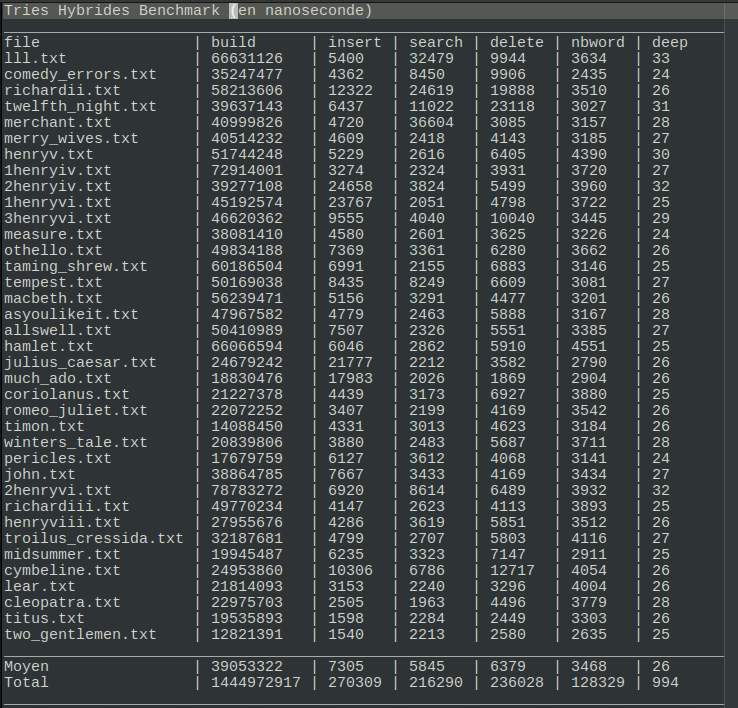
\includegraphics[scale=0.5]{BenchmarkPatc.png}

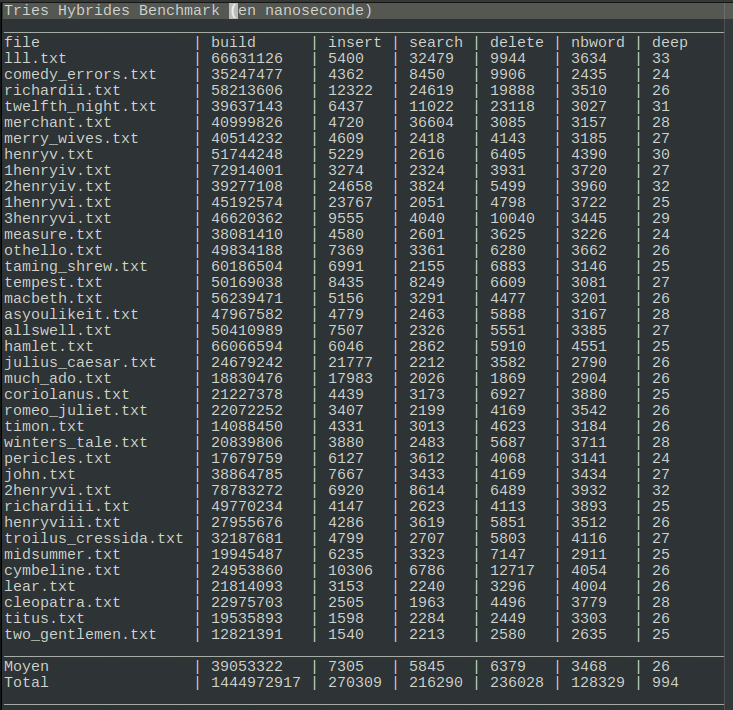
\includegraphics[scale=0.5]{BenchmarkHybc.png}

\newpage

\section{Conclusion :}

Sur quelque instance le Patricia-Tries est meilleur que le Hybride-Tries,
n\'eanmoins, en moyen l'Hybride est moins performent en construction mais ensuite
il est plus rapide que le Patricia-Tries pour les fonctions d'insertion,
d'ajout, de suppression et de recherche\\

\end{document}